\begin{minipage}[t]{0.49\linewidth}\centering
{\large\bfseries LLM + RAG}\par\smallskip
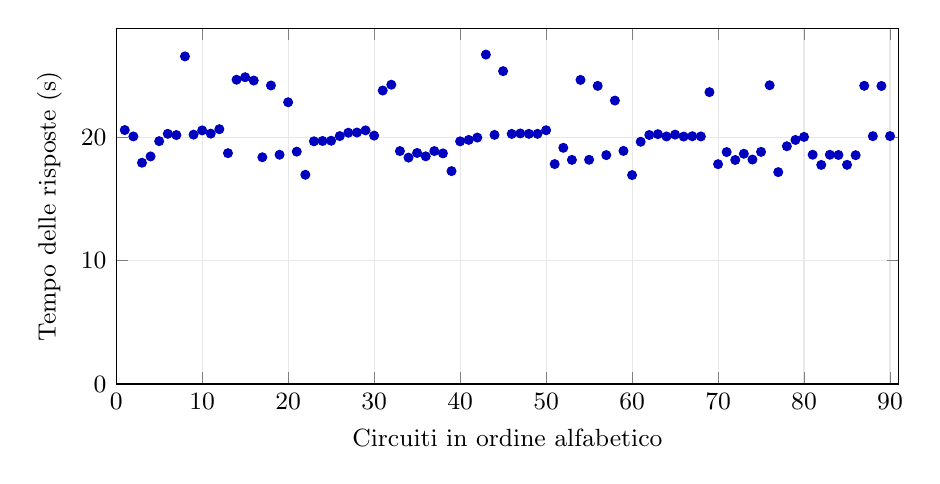
\begin{tikzpicture}\begin{axis}[width=0.95\linewidth,height=6.1cm,grid=major,grid style={gray!18},tick label style={font=\small},label style={font=\small},scaled ticks=false,/pgf/number format/use comma,unbounded coords=discard,xlabel={Circuiti in ordine alfabetico},ylabel={Tempo delle risposte (s)},xmin=0,xmax=91,ymin=0,ymax=28.86341313672013,]
\addplot[color=blue!75!black,mark=*,mark size=1.6pt,only marks] coordinates {(1,20.602634473000023) (2,20.08583998100005) (3,17.951784088000068) (4,18.462882314000012) (5,19.70408824200001) (6,20.29614488900006) (7,20.196412488999954) (8,26.580204586999912) (9,20.230536579000045) (10,20.574737945000038) (11,20.311662465999916) (12,20.674507626000036) (13,18.72790098900009) (14,24.685241054000016) (15,24.88854293600002) (16,24.618583058000127) (17,18.395355351000035) (18,24.217884013000116) (19,18.600985981999997) (20,22.858351720000087) (21,18.850340692999907) (22,16.97523269600015) (23,19.690883830000075) (24,19.71610998699998) (25,19.735992099999976) (26,20.113933981999935) (27,20.38589560100013) (28,20.40227224599994) (29,20.575702704999912) (30,20.152032730999963) (31,23.80955677599991) (32,24.28020074699998) (33,18.89857482499997) (34,18.36801526299996) (35,18.745056260999945) (36,18.471912430999964) (37,18.89911086799998) (38,18.710235494000017) (39,17.272970848999876) (40,19.68865422099998) (41,19.80287860800013) (42,19.99336547500002) (43,26.72538253400012) (44,20.211477454000033) (45,25.381958619999978) (46,20.290031054999872) (47,20.326723699000013) (48,20.29625073300008) (49,20.295892009) (50,20.5870310360001) (51,17.842763533999914) (52,19.162408244999824) (53,18.18090921399994) (54,24.67030873299973) (55,18.190897439000082) (56,24.1857306229997) (57,18.56864805400005) (58,22.99522721800031) (59,18.910006780000003) (60,16.94944505600006) (61,19.65283967000005) (62,20.201968098999714) (63,20.268203976000223) (64,20.081386432000272) (65,20.231992065000213) (66,20.075859331000174) (67,20.099900071999855) (68,20.087193501) (69,23.678153156000008) (70,17.83482659800029) (71,18.81672799800026) (72,18.17593800099985) (73,18.678450136000265) (74,18.20979908399977) (75,18.83316310600003) (76,24.235369196999727) (77,17.189952992000144) (78,19.290097365999827) (79,19.799073365999902) (80,20.046028604000185) (81,18.6012051849998) (82,17.774295488999996) (83,18.599053727999944) (84,18.580321851000008) (85,17.78302622299998) (86,18.56343483699993) (87,24.193403172000217) (88,20.10609490500019) (89,24.178653842000585) (90,20.113471841999853)};
\end{axis}\end{tikzpicture}
\end{minipage}
\hfill\begin{minipage}[t]{0.49\linewidth}\centering
{\large\bfseries LLM no RAG}\par\smallskip
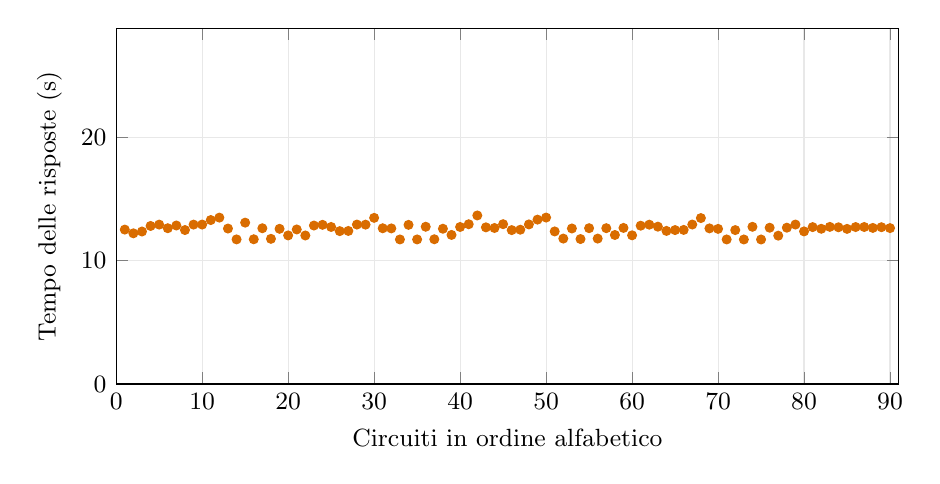
\begin{tikzpicture}\begin{axis}[width=0.95\linewidth,height=6.1cm,grid=major,grid style={gray!18},tick label style={font=\small},label style={font=\small},scaled ticks=false,/pgf/number format/use comma,unbounded coords=discard,xlabel={Circuiti in ordine alfabetico},ylabel={Tempo delle risposte (s)},xmin=0,xmax=91,ymin=0,ymax=28.86341313672013,]
\addplot[color=orange!85!black,mark=*,mark size=1.6pt,only marks] coordinates {(1,12.528046679999534) (2,12.225707725000575) (3,12.372061992999988) (4,12.821963796000091) (5,12.932124650000333) (6,12.638752882000517) (7,12.859434270999373) (8,12.492319928999677) (9,12.932523031999153) (10,12.935726771999725) (11,13.301645355999426) (12,13.498577923000084) (13,12.61290749300042) (14,11.731528495999555) (15,13.091759705000186) (16,11.743073600999196) (17,12.635741733000032) (18,11.778229237999767) (19,12.590068573999815) (20,12.05541516500034) (21,12.537792482999976) (22,12.050332731999333) (23,12.8569370969999) (24,12.914284251999561) (25,12.740294498999901) (26,12.403398207999999) (27,12.41749847399933) (28,12.935734886999853) (29,12.928787107999597) (30,13.47948869100037) (31,12.636059514000408) (32,12.623287591999542) (33,11.727144706000217) (34,12.910890326999834) (35,11.72911648200079) (36,12.758433721000074) (37,11.743161069000053) (38,12.597281972000019) (39,12.094095262000337) (40,12.74026353499994) (41,12.961504978999983) (42,13.673614674000419) (43,12.710126841000601) (44,12.658166178999636) (45,12.965845875999548) (46,12.485784727999999) (47,12.517556933999913) (48,12.94775311400008) (49,13.3354890290002) (50,13.503712988000188) (51,12.377253278999888) (52,11.797654254000008) (53,12.617964136999944) (54,11.760310643999219) (55,12.641034428999774) (56,11.797758992999661) (57,12.642082772000322) (58,12.090042155000447) (59,12.663753015000111) (60,12.062880661000236) (61,12.842801402000077) (62,12.926490358000592) (63,12.764866346999952) (64,12.420188774000053) (65,12.48785963499995) (66,12.50199932600026) (67,12.93818088199987) (68,13.462454123000498) (69,12.625960681999459) (70,12.584669705000124) (71,11.727920870000162) (72,12.48812438799996) (73,11.725788579999971) (74,12.753335964000144) (75,11.7245010609995) (76,12.679314420000082) (77,12.03496639199966) (78,12.681549914000243) (79,12.937229199000285) (80,12.381452634000198) (81,12.72876485300003) (82,12.59355984800004) (83,12.748104625999986) (84,12.714836674000253) (85,12.585746257999745) (86,12.733868976999474) (87,12.737708548000228) (88,12.664448239000194) (89,12.721447627000089) (90,12.648088394999832)};
\end{axis}\end{tikzpicture}
\end{minipage}
\par\vspace{0.45cm}\begin{minipage}[t]{0.49\linewidth}\centering
{\large\bfseries MQT Predictor}\par\smallskip
\parbox[c][6.1cm][c]{\linewidth}{\centering\large Non applicabile\\[5pt]\normalsize Questo sistema non usa un LLM.}
\end{minipage}
\hfill\begin{minipage}[t]{0.49\linewidth}\centering
{\large\bfseries Random}\par\smallskip
\parbox[c][6.1cm][c]{\linewidth}{\centering\large Non applicabile\\[5pt]\normalsize Questo sistema non usa un LLM.}
\end{minipage}
\par\vspace{0.45cm}